\chapter{Preliminaries}
\label{ch:2}

%\section{Preliminaries}
In this chapter, we introduce concepts of RDF, Wikidata, SPARQL and GraphQL. We then discuss some important differences that exist between SPARQL and GraphQL.
%\stepcounter{section}
%\setcounter{secnumdepth}{2}
\section{Resource Description Framework (RDF)}
%\subsection{RDF}
The World Wide Web consists of data published in various formats such as PDF, CSV and many forms of plain text~\cite{Ruth2013}. Linked Data is a set of principles that aims to connect and share structured data on the Web. It helps to form the Web into a global database that creates meaningful networks of information where data can be reused and shared. 

The Resource Description Framework (RDF) is a standard framework used to represent information available in the Web in the form of Linked Data. It is also considered to be the data model of Semantic Technologies and of the Semantic Web.

Structurally RDF is a graph based data model. It is used for describing and exchanging graphs over the Web. The graphs specified by RDF are directed edge-labelled graphs. This means that the edges connect source nodes to target nodes, and have labels. The graphs are a restricted form of multi-graphs. This implicates that there can be multiple edges between the same nodes. However, these edges must have different labels. Figure~\ref{fig:2} shows the representation of some extensive knowledge about the chemical element helium (extracted from the Wikidata knowledge graph) using a directed edge-labelled graph. The graph conveys the following information:\\
\hspace*{0.25cm} \textit{"Helium is a type of chemical element that has the chemical formula He. It has a boiling point, melting point and density of $-268.9^\circ\text{C}$, $-272.05^\circ\text{C}$ and $0.1785\text{kg}/\text{m}^{3}$ respectively. Helium has a discoverer/inventor by the name of Pierre Janssen whose place of birth is Paris which belongs to the country of France."}\\
\begin{figure}[h]
  \centering
  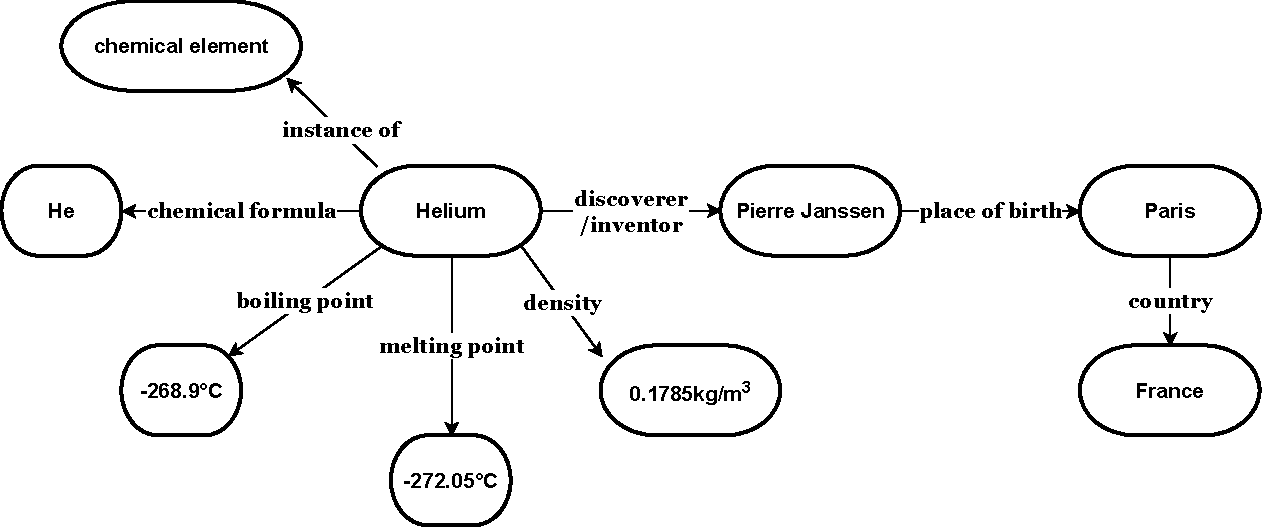
\includegraphics[width=0.95\linewidth]{images/del_graph.drawio.pdf}
  \caption{A directed edge-labelled graph describing helium}
  \label{fig:2}
\end{figure}

The technical or formal representation of graphs in RDF makes use of some important terms - IRIs, RDF literals and blank nodes. We discuss these briefly before providing a formal definition of RDF graphs.

\subsection{Internationalized Resource Identifier (IRI)}
%\subsubsection{IRIs}

In order to exchange graphs across the web we need to identify resources uniquely. For this identification, we use identifiers in RDF called IRIs. 

An Internationalized Resource Identifier (IRI) is a generalized form of URI that helps to distinguish resources with Unicode. A Uniform Resource Identifier (URI) is a sequence of a subset of ASCII characters that identifies any web resource by using a name, a location, or both. It has a scheme, authority, path, and query and fragment, where all parts other than scheme and path are optional. URIs are of the form \texttt{scheme:[//authority]path[?query][\#fragment]}. 
%\acrshort{URL}
Since in IRIs the character set of URIs is extended to the Universal Coded Character Set, IRIs can contain any Latin and non-Latin characters. This excludes some reserved characters such as \texttt{\#} and \texttt{@}. For example, \texttt{http://www.wikidata.org/entity/Q560} is an IRI that identifies the chemical element \textit{helium} in Wikidata. A Uniform Resource Locator (URL) is a subset of URI that is used to specify the location of a digital document.
%\acrshort{IRI}

An IRI is used to identify resources and properties that appear as nodes and edge labels respectively in RDF graphs. There are several pre-existing IRIs available for common use. For example, \texttt{http://www.w3.org/2000/01/rdf-schema\#label} (\textit{rdfs:label} for short) is a commonly used property in RDF to identify a resource or property with a label. New domain specific IRIs can be created based on the application. However, we must ensure there are no conflicts with other IRIs available on the web.

\subsection{RDF Literals}
%\subsubsection{RDF Literals}
\label{subsec:rdf-literals}

Data values in RDF, also known as RDF literals, are not represented by IRIs. They do not need to be identified uniquely since they share the same meaning in every application. RDF literals represent resources that have values belonging to some datatype. Each literal can have only one datatype associated to it. RDF literals are written in the format \texttt{"lexical value"\textasciicircum \textasciicircum datatype-IRI}, where lexical value is a string and datatype is an IRI. For example, the boiling point of helium is represented as \texttt{-268.9\textasciicircum \textasciicircum http://www.w3.org/2001/XMLSchema\#decimal} (\textit{-268.9\textasciicircum \textasciicircum xsd:decimal} for short) in RDF. We use rectangular nodes in graphs for RDF literals.

The W3C standard XML Schema defines datatypes and their IRIs.\footnote{www.w3.org/TR/2014/REC-rdf11-concepts-20140225/\#section-Datatypes} There are different XML Schema built-in datatypes in RDF such as string, Boolean, decimal and integer, and all of them have their own defined IRIs. For example, decimals are identified by the IRI \texttt{http://www.w3.org/2001/XMLSchema\#decimal}. 

Datatypes in RDF are specified by three components – value space, lexical space and lexical-to-value mapping. The value space is the set of all possible values that a datatype can have. A lexical value is a string\footnote{RDF is based on Unicode strings} that corresponds to a particular literal value in the value space. The lexical space contains a set of strings that are used to denote the values of the datatype. Lastly, the lexical-to-value mapping is a function that maps each string in the lexical space to an element in the value space. 

For instance, the datatype boolean has the set \texttt{{true, false}} in the value space and the set \texttt{{true, false, 1, 0}} in the lexical space. The strings \texttt{true} and \texttt{1} from the lexical space are mapped to \texttt{true} that belongs to the value space. Similarly, the strings \texttt{false} and \texttt{0} are mapped to \texttt{0}. 

In RDF, we can use a language-tagged string to denote a string in a specific language. This helps to provide human-readable labels to RDF literals. A language-tagged string is of the form \texttt{"string"@language}.\footnote{Here language is a well-formed language tag (after BCP47)} For example, the label for helium in French langauge is \texttt{hélium}, and is denoted as \texttt{"hélium"@fr} in RDF. We normally ignore the datatype-IRI for strings \texttt{(http://www.w3.org/1999/02/22-rdf-syntax-ns\#langString)} when representing string literals. 

%\acrshort{bnodes}
\subsection{Blank Nodes}
%\subsubsection{Blank Nodes}
Blank nodes in RDF, also known as bnodes, do not identify specific resources as IRIs or literals do. They are used as placeholders for some nodes, i.e., to say that something exists at the position, without specifying what the node actually is. Figure~\ref{fig:3} shows the use of a blank node in RDF. The information for address is of multi-component structure and we use a blank node in its place. The domain \texttt{http://example.org} is an example domain and does not identify a real RDF data source.

\begin{figure}[h]
  \centering
  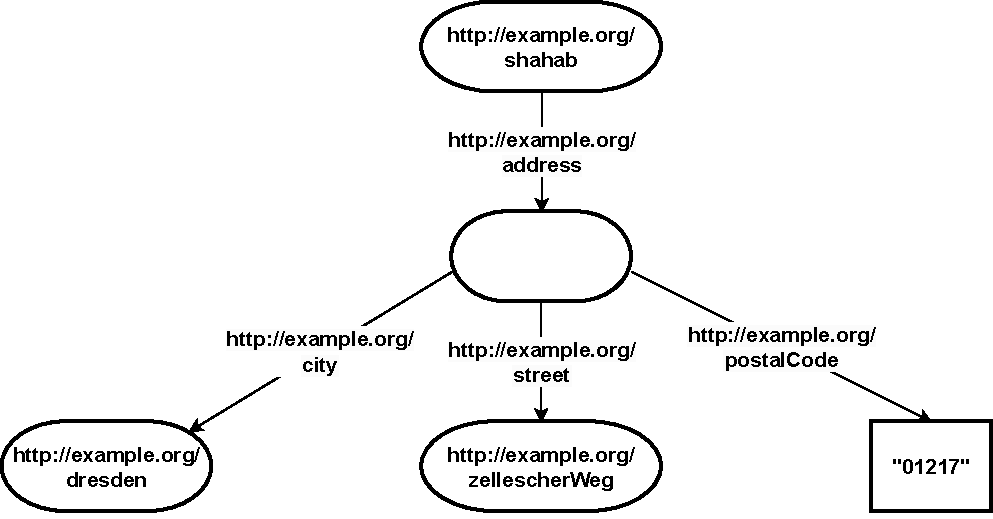
\includegraphics[width=0.80\linewidth]{images/blank_node.drawio.pdf}
  \caption{Example of a blank node in RDF}
  \label{fig:3}
\end{figure}

\subsection{RDF Graph}
\label{subsec:rdf-graph}
\begin{definition}[RDF Graph]	
An RDF graph is a directed edge-labelled graph composed of a set of triples. A triple, also known as statement, represents the relationship between a subject and an object, linked by a predicate. The subject and object nodes are the source and destination nodes respectively. Formally, each triple consist of the following elements:   

\begin{itemize}
	\item A subject node that is an IRI or a blank node.
	\item A predicate edge that is an IRI.
	\item An object node that is an IRI, a blank node, or a literal.
\end{itemize}	

\end{definition}

Figure~\ref{fig:4} shows the RDF graph of our example represented in Figure~\ref{fig:2}. We use the \texttt{http://www.w3.org/2000/01/rdf-schema\#label} property in RDF to provide a human-readable version of a resource's name.

\begin{figure}[h]
  \centering
  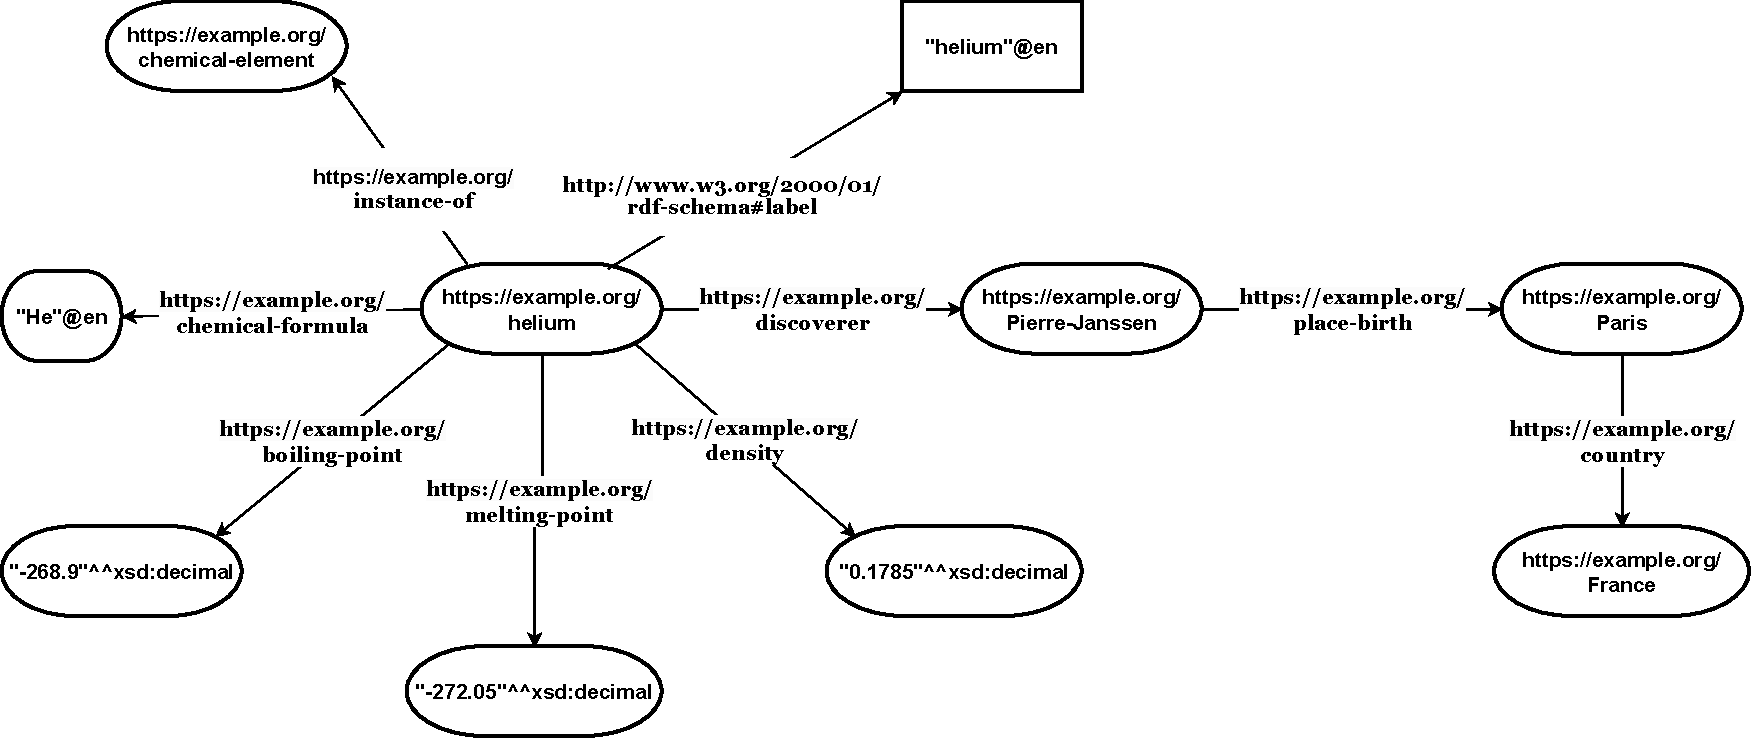
\includegraphics[width=\linewidth]{images/rdf_graph_updated.drawio.pdf}
  \caption{An RDF graph representing information about helium}
  \label{fig:4}
\end{figure}

In RDF, IRIs and literals denote resources, also called entities. In Chapter~\ref{ch:1}, we defined entities to be real world objects and abstract concepts. The predicate edge is also denoted by an IRI and represents a property. In other words, it represents a binary relation between the entities. RDF defines some resources and properties using its vocabulary. An RDF vocabulary is a collection of IRIs that we can use in RDF graphs. The RDF vocabulary is defined in the namespace \texttt{http://www.w3.org/1999/02/22-rdf-syntax-ns\#}, normally prefixed as \textit{rdf:}. For example \textit{rdf:HTML} and \textit{rdf:type} are RDF vocabularies.

RDF Schema (RDFS) extends the RDF vocabulary and is defined in the namespace \texttt{http://www.w3.org/2000/01/rdf-schema\#}, prefixed as \textit{rdfs:}. For example \textit{rdfs:class} and \textit{rdfs:label} are vocabularies defined in RDFS. RDFS provides mechanisms that allow for the depiction of groups of interconnected resources and their interrelationships. Resources can be divided into groups known as classes, and classes themselves are also resources~\cite{Brickley2014}. 

A resource belonging to a class is known to be an instance of that class. The property \textit{rdf:type} is used to represent this via the statement \textit{"X rdf:type Y"}, describing X to be an instance of Y. We recall that an RDF triple is called a statement. For example, from the RDF graph in Figure~\ref{fig:4} we see that \textit{Helium} (\texttt{https://example.org./helium}) is an instance of the class \textit{chemical element} (\texttt{https://example.org./chemical-element}) represented the property \textit{rdf:type} (\texttt{http://www.w3.org/2000/01/rdf-schema\#type)}. 


%\begin{table}[b!]
%	\begin{center}
%		\caption{Abbreviation/IDs and their meanings.}
%		\label{tab: table 1}
%		\begin{tabular}{c|c}
%%			\textbf{Benchmarking tool} & \textbf{Resource monitoring tool} & \textbf{License} & \textbf{Updated} \\ \hline
%			wd & http://www.wikidata.org/entity/ \\ \hline
%			wdt & http://www.wikidata.org/prop/direct/ \\ \hline
%			rdfs & http://www.w3.org/2000/01/rdf-schema\# \\ \hline
%			Q560 & Helium \\ \hline
%			Q298581	& discoverer/inventor \\ \hline
%			Q90 & Paris \\ \hline
%			P31	& instance of \\ \hline
%			P274 & chemical formula \\ \hline
%			P2102 & boiling point \\ \hline
%			P2101 & melting point \\ \hline
%			P2054 & density \\ \hline
%			P61	& discoverer/inventor \\ \hline
%			P19	 & place of birth \\ \hline
%			P625 & coordinate location
%		\end{tabular}
%	\end{center}
%\end{table}


\subsection{Serialisations}
For exchanging graphs across the web, we need a syntactical representation of RDF. There are different formats available~\cite{W3C2011}, the most common ones are N-Triples, Turtle, JSON-LD, RDF/XML and RDFa. In this report, we focus on N-Triples and Turtle.

\subsubsection*{N-Triples}
N-Triples~\cite{Beckett} represents RDF graphs in a simple line-based format. Every triple is encoded in a single line. The IRIs are written within pointy brackets and literals are written as \texttt{"lexical value"\textasciicircum \textasciicircum datatype-IRI}. Blank nodes are represented as \textit{\_:stringID}, where stringID can be any string used to identify the blank node in the document. After every element of a triple there is a whitespace, and all the lines end with a dot. We can use comments using hash symbol after the end of every triple in a line or in a single dedicated line, and they are treated as white spaces. N-triples files are saved with a \textit{.nt} extension.

Listing~\ref{lst:1} shows the representation of the RDF graph in Figure~\ref{fig:4} in N-triples format. We included line breaks for better readability.

\begin{minipage}{\linewidth}
\begin{lstlisting}[columns=fullflexible, label=lst:1, caption={RDF graph represented in N-triples syntax}, language=SPARQL]
<https://example.org/helium> <http://www.w3.org/2000/01/rdf-schema#type>
%\phantom{<http://www.wikidata.org/entity/Q560> <http://www.}%<https://example.org/chemical-element> .
		                                                
<https://example.org/helium> <http://www.w3.org/2000/01/rdf-schema#label> "helium"@en .

<https://example.org/helium> <https://example.org/chemical-formula> "He"@en .

<https://example.org/helium> <https://example.org/boiling-point> 
%\phantom{<http://www.wikidata.org/entity/Q560> <http://www.}%"-268.9"^^<http://www.w3.org/2001/XMLSchema#decimal> .

<https://example.org/helium> <https://example.org/melting-point> 
%\phantom{<http://www.wikidata.org/entity/Q560> <http://www.}%"-272.05"^^<http://www.w3.org/2001/XMLSchema#decimal> .

<https://example.org/helium> <https://example.org/density> 
%\phantom{<http://www.wikidata.org/entity/Q560> <http://www.}%"0.1785"^^<http://www.w3.org/2001/XMLSchema#decimal> .

<https://example.org/helium>  <https://example.org/discoverer> <https://example.org/Pierre-Janssen> .

<https://example.org/Pierre-Janssen> <https://example.org/place-birth> <https://example.org/Paris> .

<https://example.org/Paris> <https://example.org/country> <https://example.org/France> .
\end{lstlisting}
\end{minipage}

\subsubsection*{Turtle}
\label{subsubsec:turtle}
Turtle~\cite{D.Beckett} is an easy to read representation of RDF graphs. It extends the N-Triples format by providing several simplifications. We can use prefix (\texttt{PREFIX}) declarations and base namespaces \texttt{(BASE)} at the beginning of the file to shorten IRIs. This allows us to avoid repetition. We can use a semicolon at the end of a line instead of a dot if we know the next line has the same subject. Consequently, the next line will only have a predicate and object, omitting the subject. Also, we can use a comma at the end of a line if we know the next line will start with the same subject and predicate. Analogously, the next line will only have a an object omitting the subject and the predicate. 

Blank nodes are represented using only square brackets. Additionally, we can provide predicate-object pairs within the square brackets to give further triples keeping the blank node as the subject. Turtle also provides a shorthand syntax for writing numbers. Numbers of the datatype integer, decimal and double can be written without quotes and datatype-IRIs. Boolean values can be written directly as either \texttt{true} or \texttt{false}. Turtle files are saved with a \texttt{.ttl} extension.

Listing~\ref{lst:2} shows the representation of the RDF graph in Figure~\ref{fig:4} in Turtle format. 

\begin{minipage}{\linewidth}
\begin{lstlisting}[label=lst:2, columns=fullflexible, caption={RDF graph represented in Turtle syntax}, language=SPARQL]
BASE <https://example.org/>
PREFIX rdfs: <http://www.w3.org/2000/01/rdf-schema#>
PREFIX rdf: <http://www.w3.org/2000/01/rdf-schema#>
PREFIX xsd: <http://www.w3.org/2001/XMLSchema#>

<helium> rdf:type <chemical-element> ;
%\phantom{wd:Q560 }% rdfs:label "helium"@en ;
%\phantom{wd:Q560 }% <chemical-formula> "He"@en ;
%\phantom{wd:Q560 }% <boiling-point> -268.9 ;
%\phantom{wd:Q560 }% <meling-point> -272.05 ;
%\phantom{wd:Q560 }% <density> 0.1785 ;
%\phantom{wd:Q560 }% <discoverer> <Pierre-Janssen> .
<Pierre-Janssen> <place-birth> <Paris> .
<Paris> <country> <France> .
\end{lstlisting}
\end{minipage}


\section{Wikidata}
%\subsection{Wikidata}

Wikidata is built on the RDF framework. However, it does not define its resources in terms of RDFS. Instead, it has its own data model known as Wikibase data model~\citep{MediaWiki}. This data model can be expressed in RDF but there are some important differences compared to the standard Linked Data practices that RDF follows. 

Wikidata defines its own classes and properties that are equivalent to RDF constructs. For example, to denote that the subject node is an instance of a class, Wikidata uses the \textit{instance of} property instead of the \textit{rdf:type} property in RDF. Wikidata offers an explanation for some of the standards properties in Wikidata that correspond to the ones in RDF~\cite{Foundation}. 

Unlike RDF, statements in Wikidata are ranked. Additionally, they can have annotations and references. In Section~\ref{subsec:rdf-literals} we discussed that data types in RDF are mapped to XML Schema data types. However, property types in Wikidata are not defined in terms of XML Schema types. They are defined in terms of the types of values that the properties can have. For example, the \textit{element symbol} (\texttt{https://www.wikidata.org/wiki/Property:P246}) property in Wikidata is of type String, indicating it can have values that are strings.

Resources in Wikidata are called entities, and each entity is uniquely identified by an entity ID. The next section describes Wikidata entities and statements in detail.

\subsection{Entities}
Wikidata maintains its data structure by pages. Each entity has a dedicated page for itself and is identified by an unique ID. Wikidata has mainly three types of entities – items, properties and lexemes. Other extensions can define new entity types such as MediaInfo and subentities like Form and Sense. We refer to items and properties when mentioning entities. The rest are out of the scope of this report.

Items are real-world objects, concepts or events. These generally have a page in Wikipedia. For instance, there is an English Wikipedia on helium - \texttt{https://en.wikipedia.org/wiki/Helium}. Here the item is \textit{helium} and Wikidata records facts about it in a page - \texttt{https://www.wikidata.org/wiki/Q560}. Each item is identified by a \textit{QID} - an ID prefixed with the letter \texttt{Q} followed by a number. For example, the item \textit{helium} has the \textit{QID} of \texttt{Q560}. Items in Wikidata belong to the main namespace - \texttt{http://www.wikidata.org/wiki/QID}. 

Properties describe the relationship between entities and property values. Each property in Wikidata has a datatype that specifies the type and shape of the values assigned to the property. In other words, datatypes determine which values the property can accept, such as string, quantity or time.\footnote{Wikidata provides a list of all the datatypes: https://www.wikidata.org/wiki/Special:ListDatatypes} Properties are identified by a \textit{PID} - an ID prefixed with the letter \texttt{P} followed a number. They belong to the property namespace in Wikidata - \texttt{http://www.wikidata.org/wiki/Property:PID}. 

Every entity constitutes of the following main parts - labels, descriptions, aliases, and statements. Items also have sitelinks. Labels, descriptions and aliases are multilingual which help to find the respective entity. They are used to identify them clearly, since entities are identified by IDs that are not understood by humans. Sitelinks provide links about an individual item to external pages on other Wikimedia sites such as Wikipedia. 

A statement in Wikidata consists of a claim and references. Claims are property-value pairs, which along with the entity form a RDF triple, where the entity is the subject. Claims can also contain optional qualifiers that provide some additional information for the claim. This information is in the form of property-value pairs that refer to the claim instead of the entity. References point to specific resources that support the claim of statement. They can be links to URLs or items.

An entity can have several statements for the same property, and all of them might not necessarily be important or relevant. Ranks are used as a quality factor to distinguish between several statements. A Wikidata statement can have one of three types of ranks - normal, preferred and deprecated. By default, a statement has the normal rank unless changed to preferred or deprecated. A statement with preferred rank means it should be given priority over the normal ranked statements. A deprecated rank indicates that the statement is incorrect or under discussion. Deprecated statements are kept either for the sake for completion or to prevent users from constantly adding or removing them. Wikidata has around 100 million items\footnote{https://grafana.wikimedia.org/d/000000167/wikidata-datamodel} and around 1.43 billion item statements\footnote{https://grafana.wikimedia.org/d/000000175/wikidata-datamodel-statements} as of December 2022. 

Figure~\ref{fig:5} shows an excerpt of the Wikidata page on the item \textit{helium} - \texttt{https://www.wikidata.org/wiki/Q560}. We can see helium has the \textit{QID} of \texttt{Q560}, and has labels, descriptions and aliases in different languages. It has a sitelink for the item in Wikipedia offered in 186 languages. We show one of the statements that has a claim indicating that \textit{helium} has the \textit{instance of} property with \textit{chemical element} as the value. The property-value pairs (\textit{follows, hydrogen}) and (\textit{followed by, lithium}) are qualifiers of the claim. At the time of this writing, there are no references provided for this claim. This statement hence gives us the information that \textit{"Helium is an instance of chemical element, and it comes after the element hydrogen and is followed by the element lithium"}. The statement has  the normal rank (indicated by the greyed middle portion). 

\begin{figure}[hp]
  \centering
  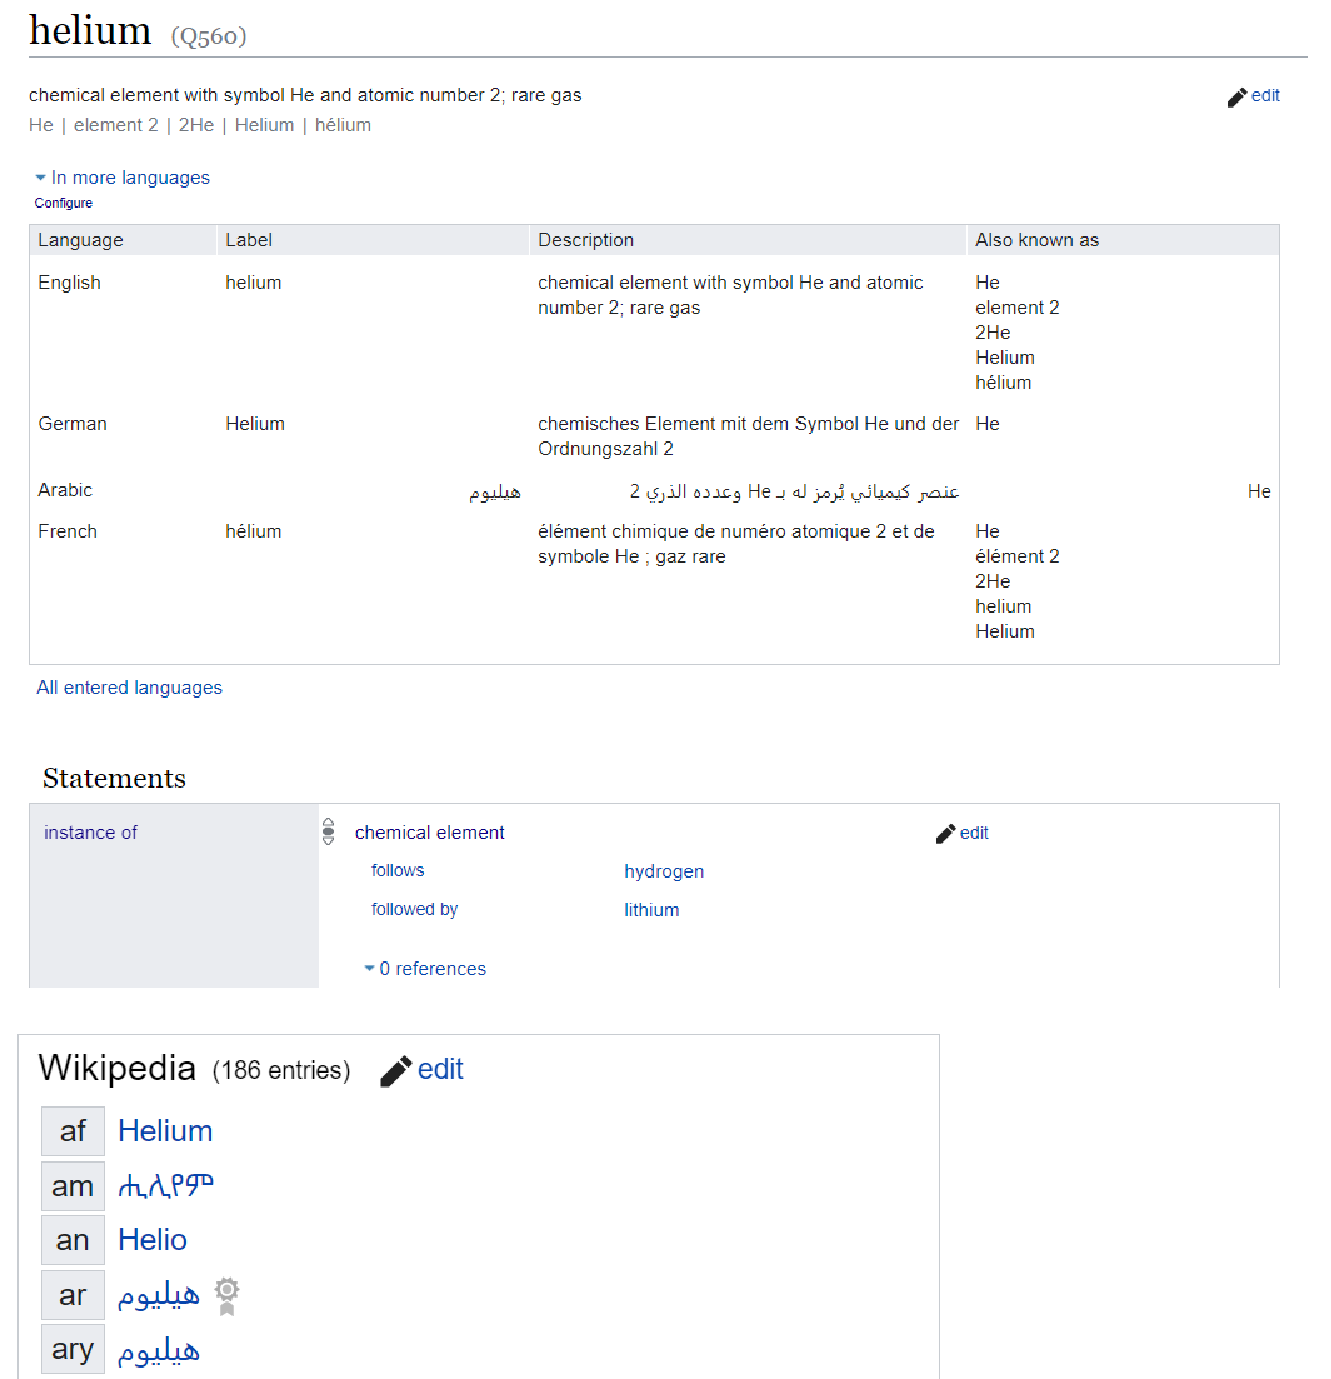
\includegraphics[width=\linewidth]{images/helium_new.pdf}
  \caption{Excerpt of the Wikidata page on helium}
  \label{fig:5}
\end{figure}

Figure~\ref{fig:6} shows an excerpt of the property \textit{instance of} page on Wikidata - \texttt{https://www.wikidata.org/wiki/Property:P31}. The property has a \textit{PID} of \texttt{P31} along and with multilingual labels, descriptions and aliases. The statement has a claim indicating that this property also has an \textit{instance of} property with \textit{Wikidata property} being the value. The rank for this statement is normal. The claim has no qualifiers and there are no references to support it. The \textit{instance of property} accepts the datatype item as a value. 


\begin{figure}[hp]
  \centering
  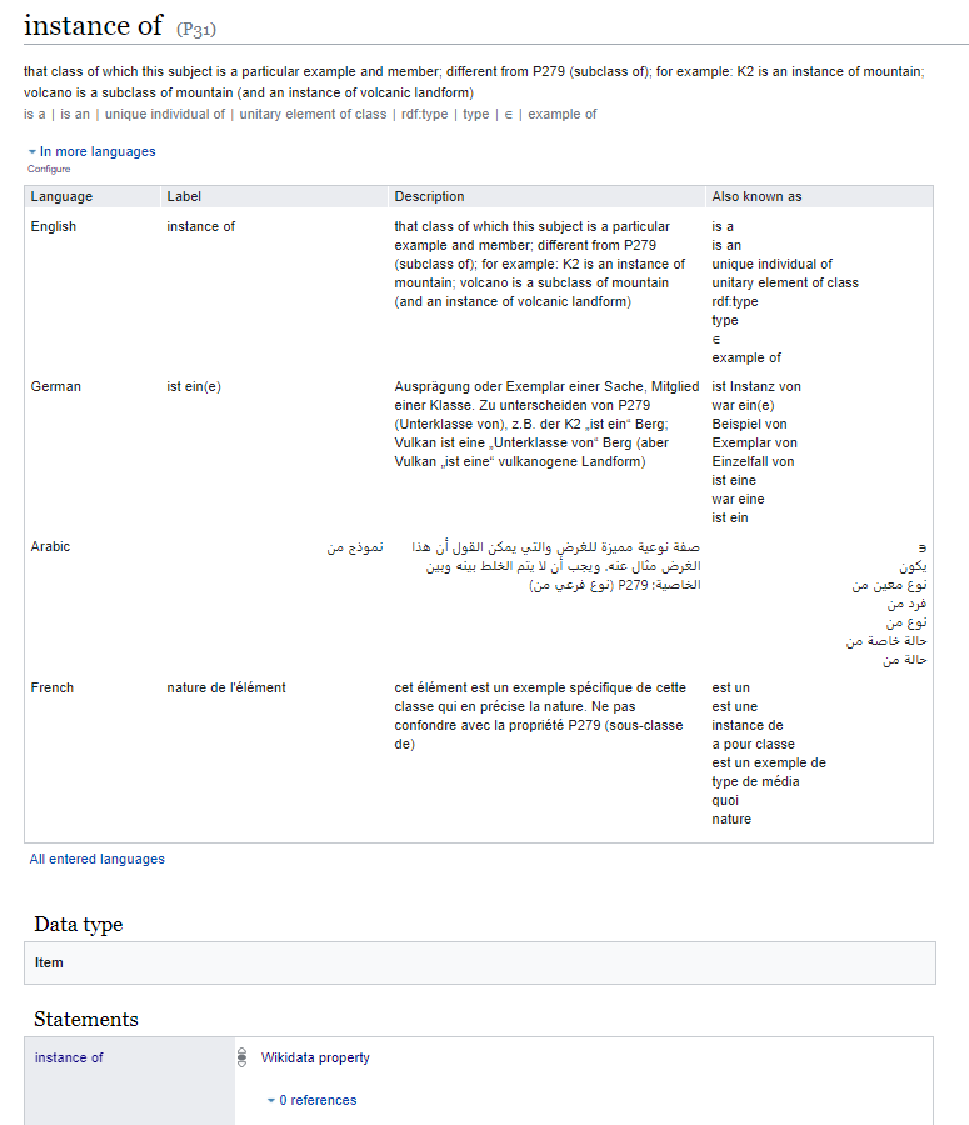
\includegraphics[width=\linewidth]{images/instance_of.pdf}
  \caption{Excerpt of the Wikidata page on \texttt{instance of}}
  \label{fig:6}
\end{figure}


The RDF graph in Figure~\ref{fig:4} used the \textit{example.org} domain and the resources identified with this domain did not point to any real data about \textit{helium}. Figure~\ref{fig:7} show information about helium, taken from Wikidata, represented in a RDF graph based on the Wikidata data model. 


\begin{figure}[h]
  \centering
  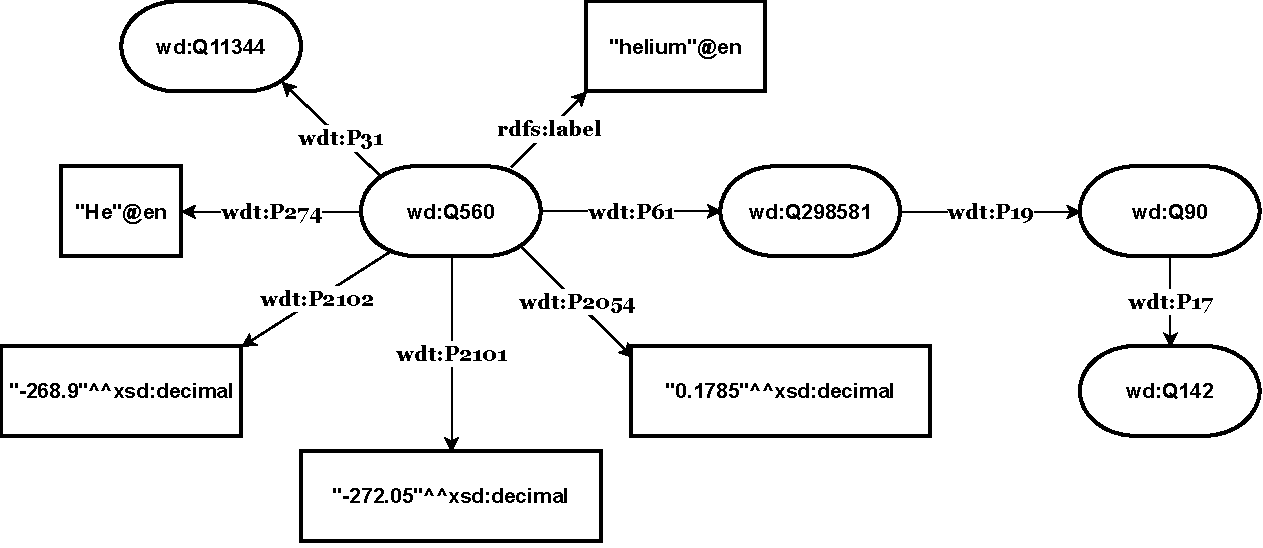
\includegraphics[width=0.75 \linewidth]{images/wikidata_graph.drawio.pdf}
  \caption{RDF graph describing the helium item in Wikidata}
  \label{fig:7}
\end{figure}

From the graphs, we see that entity nodes are represented using \textit{wd:} (prefix for \texttt{http://www.wikidata.org/entity/}) followed by the \textit{QID} for items and \textit{PID} for properties. In our example, we represent only truthy statements. This refers to statements that hold the highest rank for a given property. If any statement has a preferred rank then that statement is considered truthy, otherwise the normal ranked statements are considered truthy. Predicates for truthy statements are represented by \textit{wdt:} (prefix for \texttt{http://www.wikidata.org/prop/direct/}) followed by the \textit{PID} of the property. 

From Figure~\ref{fig:7} we understand the information that

\hspace*{0.25cm} \textit{"Helium is a type of chemical element that has the chemical formula He. It has a boiling point, melting point and density of $-268.9^\circ\text{C}$, $-272.05^\circ\text{C}$ and $0.1785\text{kg}/\text{m}^{3}$ respectively. Helium has a discoverer/inventor by the name of Pierre Janssen whose place of birth is Paris which belongs to the country of France."}\\

 \textit{Helium} \texttt{(wd:Q560)} is an \textit{instance of} \texttt{(wdt:P31)} \textit{chemical element} \texttt{(wd:Q11344)}. It has a human understandable english \textit{label}\texttt{(rdfs:label)} of \textit{helium} and has the \textit{chemical formula} \texttt{(P274)} of \textit{He}. Its \textit{boiling point} \texttt{(P2102)}, \textit{melting point} \texttt{(P2102)} and \textit{density} \texttt{(P2054)} are \textit{-268.9°C}, \textit{0.1785°C} and \textit{-272.05kg/m3} respectively. Helium has a \textit{discoverer/inventor} \texttt{(P61)} by the name of \textit{Pierre Janssen} \texttt{(Q298581)}. His \textit{place of birth} \texttt{(P19)} was \textit{Paris} \texttt{(Q90)} that belongs to the \textit{country} \texttt{(P17)} of \textit{France} \texttt{(Q142)}.

\subsection{Querying Wikidata}

The easiest and most popular way to query Wikidata is through the Wikidata Query Service (WDQS). This is Wikidata's SPARQL endpoint. We can use this service two ways. Firstly, we can write queries in SPARQL directly on the web user interface of the service\footnote{https://query.wikidata.org/} and obtain the results in different formats like table, tree, graph, etc. Secondly, the service can also be used progmatically by submitting GET or POST requests.\footnote{https://query.wikidata.org/sparql}

Another popular way to query Wikidata is by using the Wikidata API.\footnote{https://www.wikidata.org/wiki/Special:ApiSandbox} However, this API should mainly be used when we want to edit the contents of Wikidata or get data about entities like revision history.

Wikidata dumps is useful when we know our result set will be significantly large or if we want to set up our own local query service. These dumps are full exports of all the available entities in Wikidata.\footnote{https://dumps.wikimedia.org/} To get started we should download the latest complete dump.\footnote{https://dumps.wikimedia.org/wikidatawiki/latest/} Wikidata also mentions some other ways to accessing Wikidata's data like Search and Linked Data Fragments endpoint, the complete list and usage of which can be found on Wikidata's Data Access webpage~\cite{Wikidata2022}.


\section{SPARQL}
%\subsection{SPARQL}
SPARQL Protocol and RDF Query Language (SPARQL) is a W3C recommended query language for RDF. This means it allows to query any data source that can be mapped to RDF. It is also a HTTP-based protocol for linked open data on the web. This enables the transmission of SPARQL queries and results between a client and a SPARQL engine. The first working draft for SPARQL was released in 2004 and it became a W3C Recommendation in 2008~\cite{Perez2009}. 

Queries in SPARQL are based on matching graph patterns and can be used to retrieve, add or delete data in the RDF based dataset. In Section~\ref{subsec:rdf-graph} we discussed that RDF data is based on triples - subject, object and predicate. Consequently, a query in SPARQL consists of a set of triple patterns. Each of the elements of the triple can be a variable (a string beginning with \textit{"?"} or \textit{"\$"}) that needs to be queried. The solution to the variables is obtained by matching the query patterns to the triples in the dataset.

There are four forms of queries - \texttt{SELECT}, \texttt{ASK}, \texttt{CONSTRUCT} and \texttt{DESCRIBE}. 
\begin{itemize}
\item \texttt{SELECT} queries select some or all the pattern matches and provides the results in a tabular format.
\item \texttt{ASK} queries check whether there is at least one match and the result is true or false.
\item \texttt{CONSTRUCT} queries create an RDF graph based on the query results.
\item \texttt{DESCRIBE} queries return a RDF graph providing additional information on each results.
\end{itemize}

In our work, we only consider \texttt{SELECT} queries. These consist of the following major blocks:
\begin{itemize}
\item Prologue: \texttt{PREFIX} and \texttt{BASE} keywords that function similarly to those in RDF turtle format (See Section~\ref{subsubsec:turtle}).
\item Select clause: \texttt{SELECT} keyword followed by either a list of variables and variable assignments, or by *.
\item Where clause: \texttt{WHERE} keyword followed by a query graph pattern to be matched.
\item Solution set modifiers: Change the set of solutions using modifiers such as \texttt{LIMIT} and \texttt{OFFSET}.
\end{itemize}

The select and where clauses are mandatory, the rest being optional. Other optional features are filters, groups, query operators such as \texttt{UNION}, \texttt{OPTIONAL} and \texttt{BIND}, and \texttt{aggregates}.\footnote{A full specification for the query language can be found on the official W3C documentation~\cite{Seaborne}}

Listing~\ref{lst:3} shows an example of querying Wikidata using SPARQL. We want to get a list of all chemical elements, along with their English labels, that have a chemical formula, boiling point, melting point, density, an inventor/discoverer, birth place of that inventor/discoverer and the country that the place belongs to. Since there might be several results, we are limiting them to five using the \texttt{LIMIT} keyword. 


\begin{minipage}{\linewidth}
\begin{lstlisting}[label=lst:3, caption={Querying Wikidata with SPARQL}, language=SPARQL]
PREFIX wd: <http://www.wikidata.org/entity/>
PREFIX wdt: <http://www.wikidata.org/prop/direct/>
SELECT *
WHERE {
  ?element wdt:P31 wd:Q11344 ;
           wdt:P274 ?element_formula ; 
           wdt:P2102 ?boiling_point ;
           wdt:P2101 ?melting_point ;
           wdt:P2054 ?density ;
           wdt:P61 ?discoverer .
  ?discoverer wdt:P19 ?place_birth .
  ?place_birth wdt:P17 ?country .
  FILTER(LANG(?element_label)="en")
}LIMIT 5
\end{lstlisting}
\end{minipage}

The namespace \texttt{http://www.wikidata.org/entity/} is used for items when querying. We are interested in the truthy values of the properties and so the namespace \texttt{http://www.wikidata.org/prop/direct/} is used for properties. Truthy values are essentially the values for which the statement has the best non-deprecated rank. This means that if a statement has preferred rank then that statement is considered to be truthy. Otherwise, the normal ranked statement is taken to be truthy. The usage of \texttt{PREFIX} is optional since Wikidata recognizes the short forms \texttt{wd} and \texttt{wdt} automatically. We can apply the turtle syntax in SPARQL. Wikidata allows SPARQL queries to be executed in Wikidata's query service.\footnote{https://query.wikidata.org/} Table~\ref{tab:1} shows the results obtained after executing the SPARQL query.

\begin{sidewaystable}[p]
	\begin{center}
		\caption{Results of the SPARQL query in Listing~\ref{lst:3}}
		\label{tab:1}
		\renewcommand{\arraystretch}{3}
		\begin{tabular}{ccccccccc}
		
%		\textbf{element} & \textbf{element_formula} & \textbf{element_label} & \textbf{boiling_point} & \textbf{melting_point} & \textbf{density} & \textbf{discoverer} & \textbf{place_birth} & \textbf{country} \\ \hline
			\toprule
			
			\textbf{element} & \textbf{element\textunderscore formula} & \textbf{element\textunderscore label} & \textbf{boiling\textunderscore point} & \textbf{melting\textunderscore point} & \textbf{density} & \textbf{discoverer} & \textbf{place\textunderscore birth} & \textbf{country} \\ 
		
			\midrule
			
			wd:Q560 & He & helium	& -268.9 & -272.05 & 0.1785 & wd:Q298581 & wd:Q90 & wd:Q142 \\
			
			wd:Q560 & He & helium & -268.9 & -272.05 & 0.1785 & wd:Q950726 & wd:Q4093 & wd:Q145 \\ 
			
			wd:Q560 & He & helium & -268.9 & -272.05 & 0.1785	 & wd:Q127959 & wd:Q623765 & wd:Q145 \\ 
			
			wd:Q670 & Si & silicon & 4271 & 2570	& 2.329	& wd:Q151911 & wd:Q1451001 & wd:Q34 \\ 
			
			wd:Q568	& Li & lithium	& 1317	& 180.5	& 0.535	& wd:Q313568 & wd:Q10495519 & wd:Q34 \\
			
			\bottomrule

		\end{tabular}
		\renewcommand{\arraystretch}{1}
	\end{center}
\end{sidewaystable}

\section{GraphQL}
\label{sec:graphql}
GraphQL (Graph Query Language) is an open source query language for APIs (Application Programming Interfaces) and a server-side runtime for executing queries. It is data source agnostic, i.e., it is not tied to any particular data source such as a database. The data could be stored in different sources such as databases or micro-services.

With a single API call, GraphQL can aggregate data from multiple sources and resolve the data to the client. This is one of the advantages GraphQL has over REST API where the latter would require several HTTP calls to access data from multiple sources. 

GraphQL is also language agnostic. This means that GraphQL services, such as the schema and resolvers, can be written in any programming language such as JavaScript or Python. GraphQL API is usually served over HTTP through a GraphQL server. A GraphQL server consists of two main parts – schema and resolver. 

The schema defines object types that have fields. The object types represent the kind of objects that can be fetched from the data source. The fields have values that can be other object types or scalar types such as \textit{Int} or \textit{String}.\footnote{GraphQL defines some default scalar types: https://graphql.org/learn/schema/\#scalar-types} The purpose of the fields is to define the relationships between the object type and other types. This can be modelled as a directed graph where types are the nodes and fields are the edges. 

When a client sends a query request to the GraphQL server, it is parsed and the operation type is identified. The server then validates the request by checking it against the defined schema. If it fails then an error is returned otherwise the operation is executed and the resolvers process and retrieving values from the data source.

For the sake of human readability, GraphQL specification has its own Schema Definition Language (SDL). It is simple to write and understand schemas in SDL, and is similar to the language that we use to write queries. Listing~\ref{lst:4} shows a schema written in SDL. This schema can be in the GraphQL server against which clients can send queries for instances of chemical elements that have a name, chemical formula and boiling point. The exclamation mark means that the corresponding field is non-nullable and it is expected that GraphQL will give a value when the field is queried.

\begin{minipage}{\linewidth}
\begin{lstlisting}[label=lst:4, caption={A GraphQL Schema defined to query a chemical element}, language=GraphQL]
type Query {
  chemicalElement: [ChemicalElement]
}

type ChemicalElement {
  name: String!
  chemicalFormula: String!
  boilingPoint: Float!
}
\end{lstlisting}
\end{minipage}


A resolver in GraphQL server is a function that is associated with every field. It contains instructions on how to process that particular field. In other words, the resolver is responsible for retrieving a value from the data source.
 
A GraphQL query has a tree-like structure. The root node is at the top level and represents the parent node or objects. The parent node is the object type specified in the schema. The leaf nodes represent the children nodes, and are the fields of their respective object types in the schema. When describing GraphQL queries, we use the terms root node and object interchangeably, and analogously the terms leaf node and fields. To traverse the query we can follow this tree structure, i.e., we can go up to a parent node, down to a child node or left/right to a sibling node~\cite{Perez2009}. When querying the idea is to request for some fields on objects.

There are three operations types in GraphQL – \textit{query}, \textit{mutation} and \textit{subscription}. Query operations are used to fetch or read data from a data source. They are similar to GET requests in REST (Representational State Transfer). Mutation operations allow modifying data on the source by updating, adding or deleting. Subscription operations notify us about some events related to the data in a source such as addition of new data.

Listing~\ref{lst:5} shows a GraphQL query that can be used against the above schema. The query fetches the \textit{name}, \textit{chemicalFormula} and \textit{boilingPoint} of the objects returned by  the \textit{chemcalElement} node, where \textit{chemicalElement} is of type \textit{ChemialElement}. 

\begin{minipage}{\linewidth}
\begin{lstlisting}[label=lst:5, caption={GraphQL query to fetch chemical elements and their properties}, language=GraphQL]
query QueryChemicalElement {
  chemicalElement(limit: 2){
    name
    chemicalFormula
    boilingPoint
  }
}
\end{lstlisting}
\end{minipage}

Running the query against some data source provides a sample result as shown in Listing~\ref{lst:6}. The results obtained are in JSON format. We see that the shape of the results is similar to the shape of our query. This is crucial to GraphQL as we always get the type of response we expect when we write queries. Defining the types and fields in the schema allows the server to know the fields that the client can query for an object type. Also, GraphQL ensures the queries to return predictable results by providing the clients with control over the content of the data they receive. Hence, there is not over or under fetching of data.



\begin{minipage}{\linewidth}
\begin{lstlisting}[label=lst:6, caption={Results of the GraphQL query}, language=GraphQL]
{
  "data": {
    "chemicalElement": [
      {
        "name": "helium",
        "chemicalFormula": "He",
        "boilingPoint": -268.9
      },
      {
        "name": "silicon",
        "chemicalFormula": "Si",
        "boilingPoint": 4271
      }
    ]
  }
}
\end{lstlisting}
\end{minipage}

In GraphQL clients can fetch related data (fields in the query) with a single HTTP request made to the GraphQL server. This reduces network overheads and improves performance.

GraphQL offers several features that enhance its functionality to fetch data. Some important ones are summarized below.\footnote{List of all the features can be found at: https://graphql.org/learn/}

\subsection{Arguments}
In GraphQL we can pass arguments to parent nodes and fields. These can be of different types such as units for a weight field or IDs to fetch information about specific objects.

\subsection{Variables}
We can dynamically set values for arguments by the use of variables. The variables are passed by the client in the form of a dictionary. This enables querying for different arguments instead of constructing a new query every time.

\subsection{Aliases}
Aliases are used to rename the results for a parent node or a field. The purpose is to avoid conflicts that might occur when querying for the same parent or field but by passing different arguments.

\subsection{Fragments}
Fragments are reusable units for sets of fields to help avoid repetitions. We can construct a unit comprised of some fields, and include this unit each time we need it in our query.

\subsection{Inline Fragments}
Inline fragments allow us to query fields based on the type of object. It is useful when we query objects of different types and fetch different fields for each type.

\subsection{Directives}
Directives modify the behaviour of a GraphQL query or schema. They can be used on fields or fragment inclusions using the \texttt{"@"} symbol followed by the directive name and any required arguments. There are two directives that are supported by any GraphQL server compliant with official GraphQL specification:

\begin{itemize}
\item \texttt{@include(if: Boolean)} -  Conditionally includes the field in the result if the argument is true.
\item \texttt{@skip(if: Boolean)} -  Conditionally skips the field if the argument is true.
\end{itemize}

We can also define custom directives in the schema definition to provide additional functionality.

\subsection{Mutations}
Apart from fetching data, GraphQL also allows to modify data on the server. Modification refers to creation, update or deletion. This is implemented by the mutation operation. 

\subsection{Non-null type modifier}
In GraphQL we can define fields in the schema definition to be non-null. This is done by adding a non-null type modifier (the \texttt{"!"} symbol) after the type name for the field in the schema. By using the modifier we indicate that the server expects to return a non-null value for the field. An execution error is triggered if the servers gets a null value for the field. 

We can also use the modifier when defining arguments for a field in the GraphQL query. The server returns a validation error if a null value is passed as the argument. 

\subsection{Pagination}
Pagination is the technique of dividing a dataset into smaller chunks or pages. It helps in the efficiency and performance of data retrieval. The most common approach is to control the number of results returned and the offset of the first results. This is achieved by using the first and offset arguments in GraphQL.

\subsection{Introspection}
GraphQL allows us to query the GraphQL schema using the introspection system. Introspection helps to find out the types, fields and directives defined in the schema. This is useful when we want information about the queries supported by the schema.

%\begin{itemize}
%\item Arguments – Objects and fields can have arguments passed as parameters
%
%\item Aliases – The results of a field can be renamed to avoid any conflicts that might occur when querying for the same fields but with different arguments. 
%
%\item Fragments – Reusable units for sets of fields to help avoid repetitions.
%
%\item Operation name – We can set a name to our operation to help in debugging. The name must be preceded by the operation type. When no name is mentioned (as our example in Listing XYZ) the query operation is considered to be of type query 
%
%\item Variables – Set arguments to fields dynamically
%
%\item Directives – Used to modify the behavior of a field or fragment. There are two directives that must be supported by GraphQL servers: 
%
%\begin{itemize}
%\item @include(if: Boolean) -  Include the field in the result if the argument is true.
%\item @skip(if: Boolean) -  Skip the field if the argument is true.
%\end{itemize}
%
%\item Mutations – Allow to modify data
%
%\item Inline Fragments – Used to return an interface or a union type
%
%\item Meta fields – The \_\_typename meta field can be used to get the name of the object type defined in the schema
%
%
%\item Non-null – Can be used in queries and schemas to indicate that an argument or field cannot be null; specified by an exclamation mark 
%
%
%\item Interfaces – An abstract type containing a set of fields. Object types must include these fields when implementing the interface.
%
%
%\item Union types – Used to define a type that can represent several different types.
%
%\item Pagination – Used to control the number of results returned and the offset of the first results. 
%
%\item Introspection  - Query schema to find out the types, fields and directives defined in the schema
%\end{itemize}

Listing~\ref{lst:7} shows a GraphQL query to demonstrate the use of arguments, variables, aliases, fragments, directives, non-null and pagination. It also contains the variables defined.

\begin{minipage}{\linewidth}
\begin{lstlisting}[columns=fullflexible, label=lst:7, caption={GraphQL query demonstrating some useful features}, language=GraphQL]
query GetChemicalElementDetails($chemicalFormula: String!, $first: Int!, $includeBoilingPoint: Boolean!) {
	oneElement: chemicalElement(chemicalFormula: $chemicalFormula) {
		name
		chemicalFormula
		boilingPoint @include(if: $includeBoilingPoint) 
	}
	manyElements: chemicalElement (first: $first) {
	...elementFields
	}
}

fragment elementFields on ChemicalElement {
	name
	chemicalFormula
	meltingPoint
	density
}

#-------------------------------------
#variable definitions
{
	"chemicalFormula": "He",
	"first": 5, 
	"includeBoilingPoint": true
}
\end{lstlisting}
\end{minipage}

The query \textit{GetChemicalElementDetails} takes three non-null arguments as input from the client in the form of variables – \textit{\$chemicalFormula} of type "String", \textit{\$first} of type "Int" and \textit{\$includeBoilingPoint} of type "Boolean". We see in the variable definitions section the input passed.

The aliases \textit{oneElement} and \textit{manyElements} are used as we are querying the same parent node \textit{chemicalElement}. The \textit{oneElement} node queries for details about \textit{chemicalElement} objects that have the \textit{chemicalFormula} \texttt{"He"}. This node also has the field \textit{boilingPoint} that is conditionally included using the \texttt{@include} directive and is fetched when the \textit{if} argument is \texttt{true}. In this case it is included since the user passes \texttt{true}. 

The \textit{manyElements} node also queries for \textit{chemicalElement} objects. The limit for the number of objects is set by the \textit{first} argument and is set to \texttt{5}. This node uses a fragment called \textit{elementFields} to fetch details about the objects.


\section{GraphQL vs SPARQL}
There are some crucial differences that exist between GraphQL and SPARQL. We highlight some of these below.

\subsection{Goals}
GraphQL and SPARQL are query languages developed with different goals in mind. GraphQL is designed to provide an efficient and flexible way to fetch data from APIs. It solves issues that are typical with using REST APIs such as over or under fetching of data, and requiring multiple HTTPS requests to query related data. 

On the other hand, SPARQL is a query language and protocol developed for working with RDF data. It provides a standard and flexible way for querying data stored in RDF format. The data can be distributed over multiple sources. Since it is also a protocol, it allows interacting with RDF data over HTTP. 
 
\subsection{Commercial usage}
GraphQL was developed as an alternate to REST APIs and is popular among software and web developers. 
SPARQL is popular in the field of research and academia where it used for querying and analysing. However developers working with tools like JSON and REST APIs are not much aware of SPARQL~\cite{Angele2022}. They are not familiar with SPARQL queries and their triple-based output~\cite{Angele2022}. 

%GraphQL, on the other hand, is more popular among software and web developers.

%Many developers are still not familiar with the Linked Data model of RDF and SPARQL. 
%Develops are not familiar with querying with SPARQL and its triple-based output~\cite{Angele2022}. So they are unable to use full potential of knowledge graphs.

%They are more used to working with technologies such as GraphQL and RESTAPIs. 

GraphQL is simple to learn and work with since it has human-oriented syntax. This makes it easy to use in application development. SPARQL however, proves to be more complex. It has more syntactic verbosity owing to the descriptive nature of writing queries. The produced output from SPARQL queries contains a lot of unnecessary metadata that is not useful for web developers and need to be further parsed for using in web applications~\cite{Lisena2018}. 

Developers are more equipped in using nested objects that GraphQL offers~\cite{Taelman2018}. They lack the experience to work with triples which is the main foundation of SPARQL. There are fewer supporting tools and libraries for working and developing applications with SPARQL when compared to GraphQL~\cite{Taelman2018}. As a result, developers working with SPARQL may need to write more custom code as opposed to when working with GraphQL APIs. Furthermore, there is limited documentation available for proper ontology descriptions and examples of using queries for SPARQL endpoints~\cite{Angele2022}. This causes retrieval of data from knowledge graphs using SPARQL to be time consuming.

%Moreover, retrieval of data from knowledge graphs using SPARQL is time consuming and proves to be a steep learning curve, the reason being that there is limited documentation available for proper ontology descriptions and examples of using queries for SPARQL endpoints~\cite{Angele2022}. 


\subsection{Expressivity}
SPARQL queries represent full graphs while those of GraphQL represent trees~\cite{Taelman2018}. In SPARQL, we can specify patterns of triples that traverse the entire graph to retrieve data that matches a particular pattern. This allows querying for complex relationships between resources. SPARQL provides advanced features such as property paths and complex graph patterns to manipulate and query data. GraphQL queries represent data in a hierarchy as a tree-like structure. They are composed of fields that specify the data that needs to be returned. They can only retrieve data from a particular node and its descendants. As a result, SPARQL is more expressive than GraphQL.

%For example, triangle relations in a graph can be expressed in SPARQL but not in GraphQL. Consider a graph that represents students in a chemistry laboratory, where each student can follow other student in Twitter, and each student has a set of favourite chemicals. Suppose we want to retrieve all students that follow other students who share the same favourite chemicals as them. This involves traversing three entities – the follower student, the followed student and the set of favourite chemicals. In SPARQL, we can traverse the entire graph to retrieve such students. However, since GraphQL queries are tree-based and retrieve data from a particular node and its descendants, it is not possible to retrieve the students with GraphQL. 

Furthermore, in SPARQL we can query if a node is connected to another node by a path of arbitrary length, where all edges are labelled. However, GraphQL cannot implement such queries as it can only query for a path of fixed length.

RDF provides a system to build detailed structures from the meaning of data, and is hence more complete and capable than GraphQL schemas~\cite{Dresslar2019}. Since SPARQL works with the schema organization of RDF, this makes it more powerful than GraphQL. With SPARQL we can write complex queries that can be used to retrieve or modify data~\cite{Angele2022}. As a result, it is capable to satisfy many complex use cases.

\subsection{Querying multiple sources}
Since GraphQL alone has no notion of semantics~\cite{Taelman2018}, a schema needs to be defined by the GraphQL API developers for every interface they want the client to query. This makes it difficult to integrate data returned when querying multiple different sources. SPARQL however supports federated queries which makes it more powerful and rich. 